\documentclass[class=report, crop=false, 12pt,a4paper]{standalone}
\usepackage{enumitem}
\usepackage{multicol}
\usepackage{graphicx}
\usepackage{float}
\usepackage{amsmath}
\usepackage{amssymb}
\usepackage{mathtools}
\usepackage{siunitx}
\usepackage{commath}
\usepackage{array}
\usepackage{natbib}
\usepackage[a4paper,width=150mm,top=25mm,bottom=25mm]{geometry}
\setlength{\parindent}{0pt}
\begin{document}
\begin{center}
  16/10/2020
\end{center}
\section{Derivation of Bending Equations}
\subsection{Equilibrium – Beam Bending Equations}
\begin{figure}[H]
  \centering
  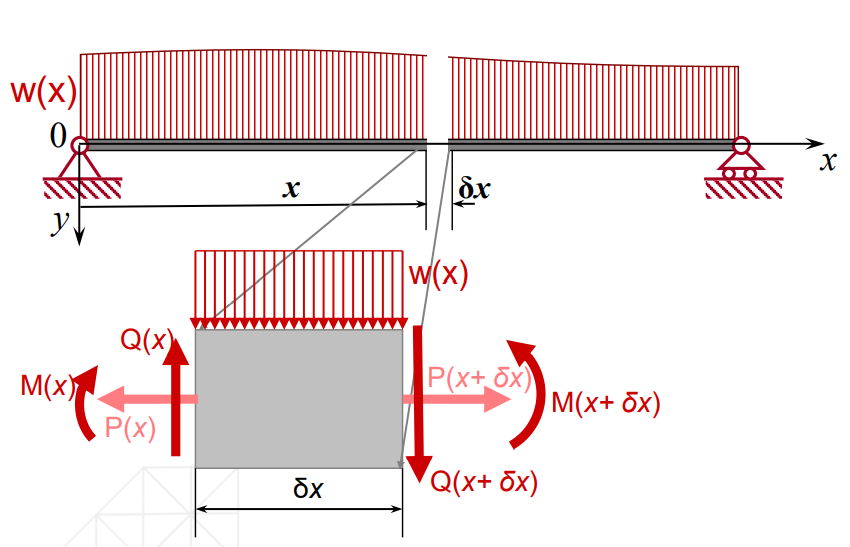
\includegraphics[width = 0.8 \textwidth]{../img/beam1.PNG}
  \caption{Horizontal beam with vertical distributed load. We focus a section of the beam with the very small length $\delta x$.}
\end{figure}
\textbf{y-direction}
\begin{gather}
  Q(x+\delta x) - Q(x) + w(x)\delta x = 0
\end{gather}
\textbf{x-direction}
\begin{gather}
  M(x+\delta x) - M(x) - Q(x)\delta x + w(x)\cdot \delta x \cdot \frac{\delta x}{2} = 0
\end{gather}
We assume that $\delta x$ is so small that no matter the distribution of the load on the beam, $w(x)$ is constant along the investigated beam section. \\\\
Rearranging the terms in the $y$ direction yields: 
\begin{gather}
  \frac{Q(x+\delta x)-Q(x)}{\delta x} = -w(x)
\end{gather}
Taking $\delta x$ to the smallest limit (0), the above equation can be written as:
\begin{gather}
  \delta x = 0 \\
  \frac{\dif Q}{\dif x} = -w(x) \\
  w(x) = -\frac{\dif Q}{\dif x}
  \label{loadiny}
\end{gather}
The load $w$ in the $y$ direction is the derivative of the shear force $Q$. Integrating equation (\ref{loadiny}):
\begin{gather}
  Q = -\int w \dif x 
\end{gather}
We consider the bending moment at the distance $\delta x$ (right-side for the example). Rearranging the terms in the $x$ direction yields: 
\begin{gather}
  \frac{M(x+\delta x)-M(x)}{\delta x} = Q(x) - \frac{1}{2}w(x)\delta x
\end{gather}
Taking $\delta x$ to the smallest limit (0), the above equation can be written as:
\begin{gather}
  \delta x = 0 \\
  Q(x) = \frac{\dif M}{\dif x} \\
  \label{momentinx}
\end{gather}
The shear force $Q$ is the derivative of the bending Moment $M$. Integrating equation (\ref{momentinx}):
\begin{gather}
  M = \int Q \dif x 
\end{gather}
\subsubsection{Example:}
\begin{figure}[H]
  \centering
  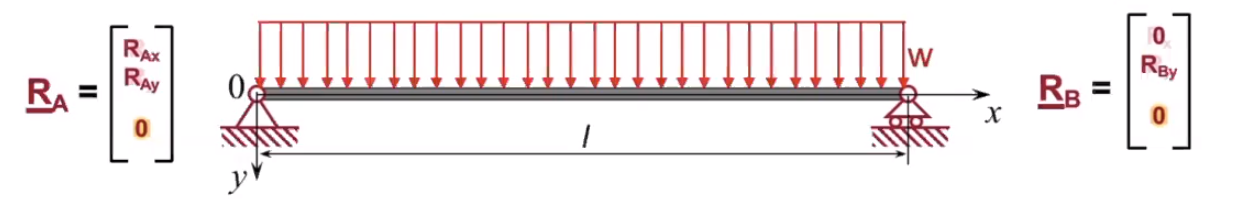
\includegraphics[width = 1 \textwidth]{../img/example1.PNG}
\end{figure}
\begin{gather}
  Q = -\int w \dif x \\
  = -wx + Q_0 \\\\
  M = \int Q \dif x \\
  = \int(-wx+Q_0)\dif x \\
  = -\frac{1}{2}wx^2 + Q_0\cdot x + M_0
\end{gather}
Applying the boundary conditions: 
\begin{gather}
  M(0) = 0 \rightarrow -\frac{1}{2}w\cdot 0^2 + Q_0\cdot 0 + M_0 = 0 \\
  M_0 = 0 \\\\
  M(l) = 0 \rightarrow -\frac{1}{2}wl^2 + Q_0\cdot l + 0 = 0 \\
  Q_0 = \frac{1}{2}wl
\end{gather}
Overall:
\begin{gather}
  Q = -wx + \frac{1}{2}wl \\
  M = -\frac{1}{2}wx^2 + \frac{1}{2}wlx
\end{gather}
\begin{figure}[H]
  \centering
  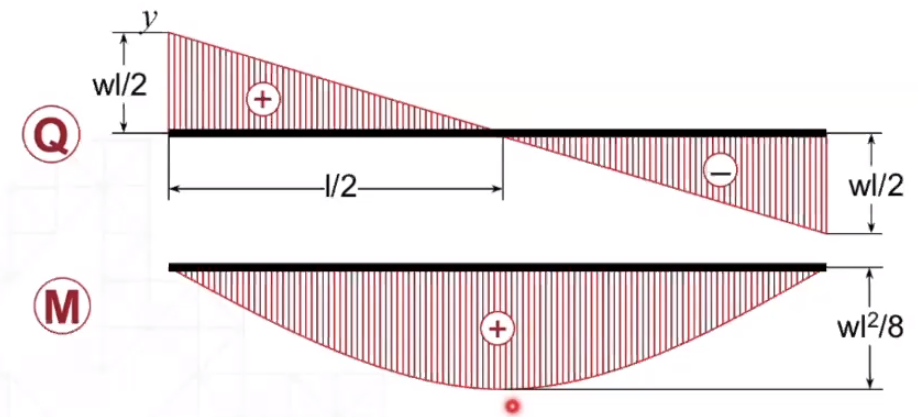
\includegraphics[width = 0.7 \textwidth]{../img/example1graphs.PNG}
  \caption{The shear force and bending moment varying along $x$}
\end{figure}
\section{Differential Equations for Deflection}
\subsection{Theory of Pure Bending}
\begin{itemize}[noitemsep]
  \item The beam is initially straight and unstressed;
  \item The beam material is perfectly homogeneous and isotropic;
  \item Plane cross-sections remain plane before and after bending;
  \item Every cross-section in the beam is symmetrical about the plane of bending;
  \item There is no resultant force perpendicular to any cross-section.
  \item The elastic limit is nowhere exceeded; 
  \item Young’s Modulus for the material is the same in tension and compression;
\end{itemize}
\subsection{Compatibility - Strains in Pure Bending}
Consider a portion of the length $\dif x$ from the beam subject to uniform bending. 
\begin{figure}[H]
  \centering
  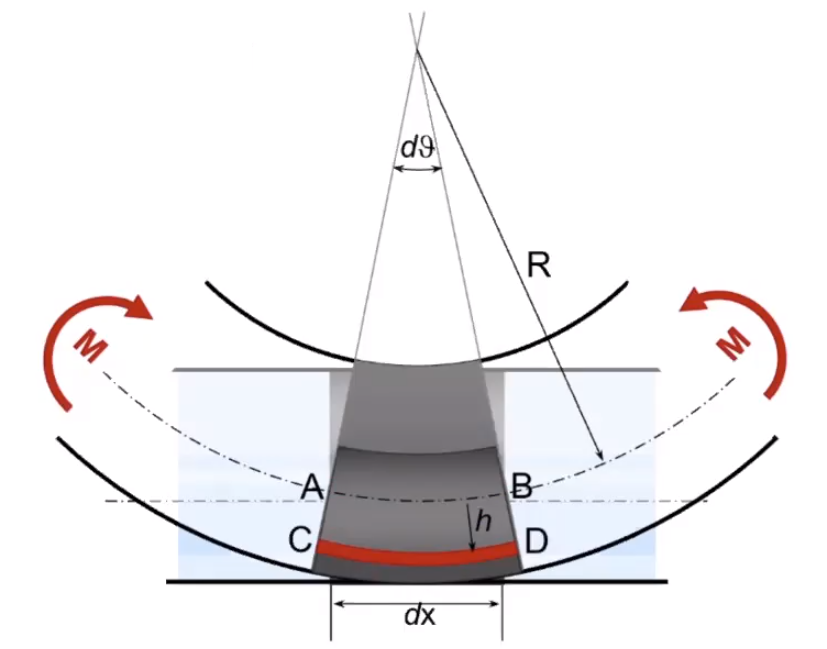
\includegraphics[width = 0.6 \textwidth]{../img/compatibility.PNG}
\end{figure}
Lower fibres stretch and upper fibres shorten. Hence, since cross-sections remain plane, there must be a plane where the fibre elongation is zero. This is called \textbf{neutral plane} (it is a plane because section is symmetrical) and the intersection with the plane of bending is called \textbf{neutral axis}. \\\\
If we indicate with $R$ the radius of curvature of the neutral axis, along the neutral plane:
\begin{gather}
  \overline{AB} = \widehat{AB} \\
  \widehat{AB} = \dif x = R\dif \theta
\end{gather}
For a generic plane CD, distant $h$ from N.A.:
\begin{gather}
  \widehat{CD} = (R+h)\dif \theta
\end{gather}
The longitudinal strain of CD is given by:
\begin{gather}
  \epsilon(h) = \frac{elongation}{initial\ length} = \frac{\widehat{CD}-\overline{CD}}{\overline{CD}} \\\\
  = \frac{(R+h)\cdot \dif \theta - R\cdot \dif \theta}{R\cdot \dif \theta} = \frac{h}{R} \\\\
  \epsilon(h) = \frac{h}{R}
  \label{epsilon}
\end{gather}
\begin{figure}[H]
  \centering
  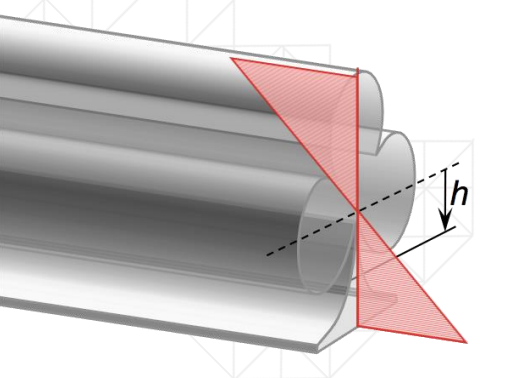
\includegraphics[width = 0.3 \textwidth]{../img/straindistribution.PNG}
  \caption{Strains are distributed linearly across the section}
\end{figure}
Stresses and strains can be associated with each other. For most materials, under small deformation:
\begin{gather}
  \sigma = E\cdot \epsilon
  \label{sigma}
\end{gather}
Where:
\begin{itemize}[noitemsep]
  \item $\sigma$ is the stress
  \item $E$ is the Young Modulus
  \item $\epsilon$ is the strain
\end{itemize}
Therefore, from equations (\ref{epsilon}) and (\ref{sigma}):
\begin{gather}
  \sigma_x(h) = E\frac{h}{R}
\end{gather}
\subsection{Constitutive - Stress-Curvature Relation}
Stress is also distributed linearly across the section, being 0 at the neutral plane and maximum (in tension and compression) at the outer surfaces, where the distance from the neutral plane is maximum. 
\begin{gather}
  \sigma_{min} = E\frac{h_{min}}{R} \\
  \sigma_{max} = E\frac{h_{max}}{R}
\end{gather}
The minimum value is at the compression and the maximum value is at the tension. This just follows the convention; the tension is taken as positive and compression is taken as negative, in terms of the stress direction.
\subsection{Equilibrium - Force-Stress Relation}
\begin{figure}[H]
  \centering
  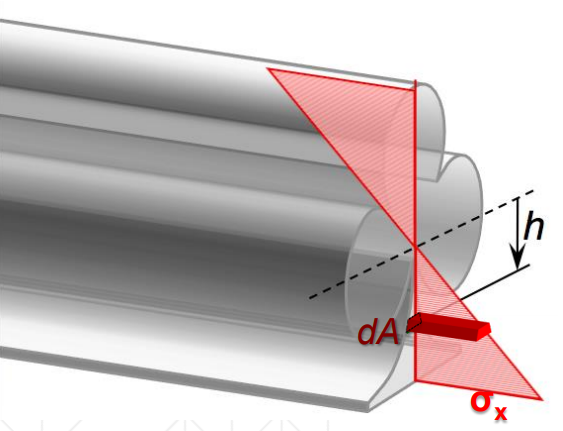
\includegraphics[width = 0.3 \textwidth]{../img/forcestressrelation.PNG}
\end{figure}
Considering an elemental area $\dif A$, the force associated with bending stress is:
\begin{gather}
  \dif F_x = \sigma_x \cdot \dif A \\
  = E\frac{h}{R}\cdot \dif A
\end{gather}
For the force equilibrium of the entire section: 
\begin{gather}
  \int_{A}\dif F_x = \int_{A} E\frac{h}{R}\cdot \dif A = 0 \\ 
\end{gather}
$E$ and $R$ are constants, so they don't affect the integral and can be taken out. Hence the first moment of area is:
\begin{gather}
  \int_{A} h\cdot \dif A = 0
\end{gather}
The first moment of area of a section is zero if it is calculated about the centroid. \textbf{The neutral axis corresponds to the centroid of the section.}
\subsection{Equilibrium - Bending-Stress Relation}
Considering an elemental area $\dif A$, the internal moment produced by the bending stress is:
\begin{gather}
  \dif M = \sigma_x \cdot h \cdot \dif A \\
  = \dif F_x \cdot h \\
  = E\frac{h}{R} \cdot h \cdot \dif A
\end{gather}
Moment of the entire section:
\begin{gather}
  M = \int_{A}\dif M = \int_{A} E\frac{h^2}{R}\cdot \dif A = \frac{E}{R}\int_{A} h^2\cdot \dif A
\end{gather}
The second moment of area is:
\begin{gather}
  \int_{A} h^2\cdot \dif A = I
\end{gather}
The second moment of area represents how easy or difficult it is to bend a beam, depending on the shape of the cross section. The overall relation is:
\begin{gather}
  M = \frac{EI}{R}
\end{gather}
This defines how the cross section, elastic modulus, curvature, and bending moment are related to each other.
\subsection{Solid Mechanics Equations}
\begin{figure}[H]
  \centering
  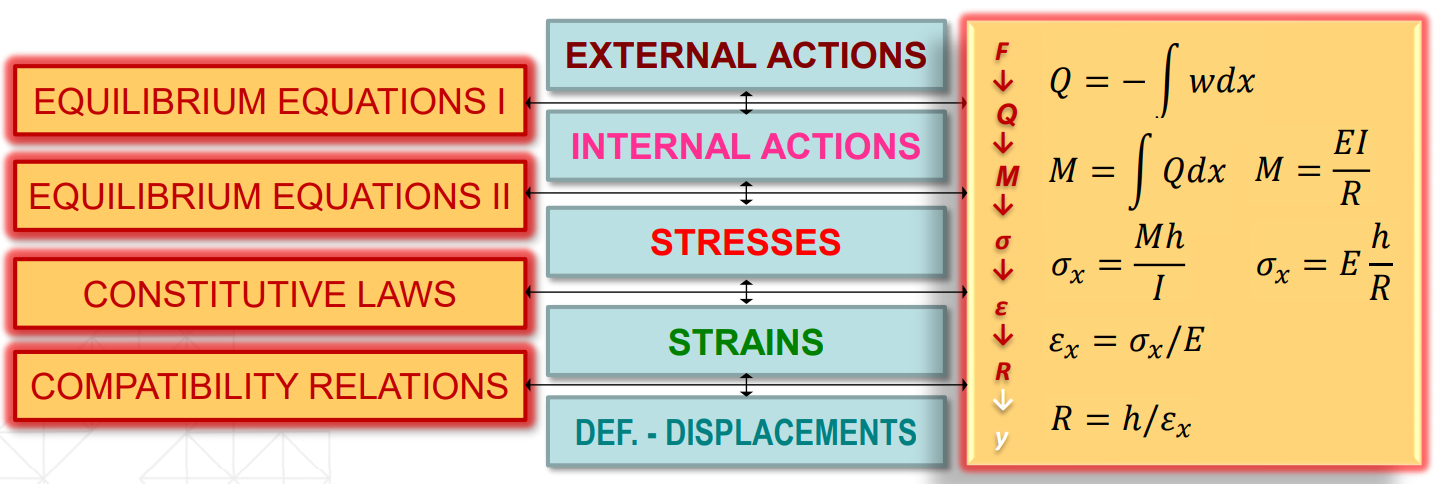
\includegraphics[width = 0.8 \textwidth]{../img/solidmechanicsequations.PNG}
  \caption{The relationships between Force, Shear Force, Bending Moment, Stress, Strain, Curvature}
\end{figure}
\subsection{Geometric - Slope-Deflection Relation}
\begin{figure}[H]
  \centering
  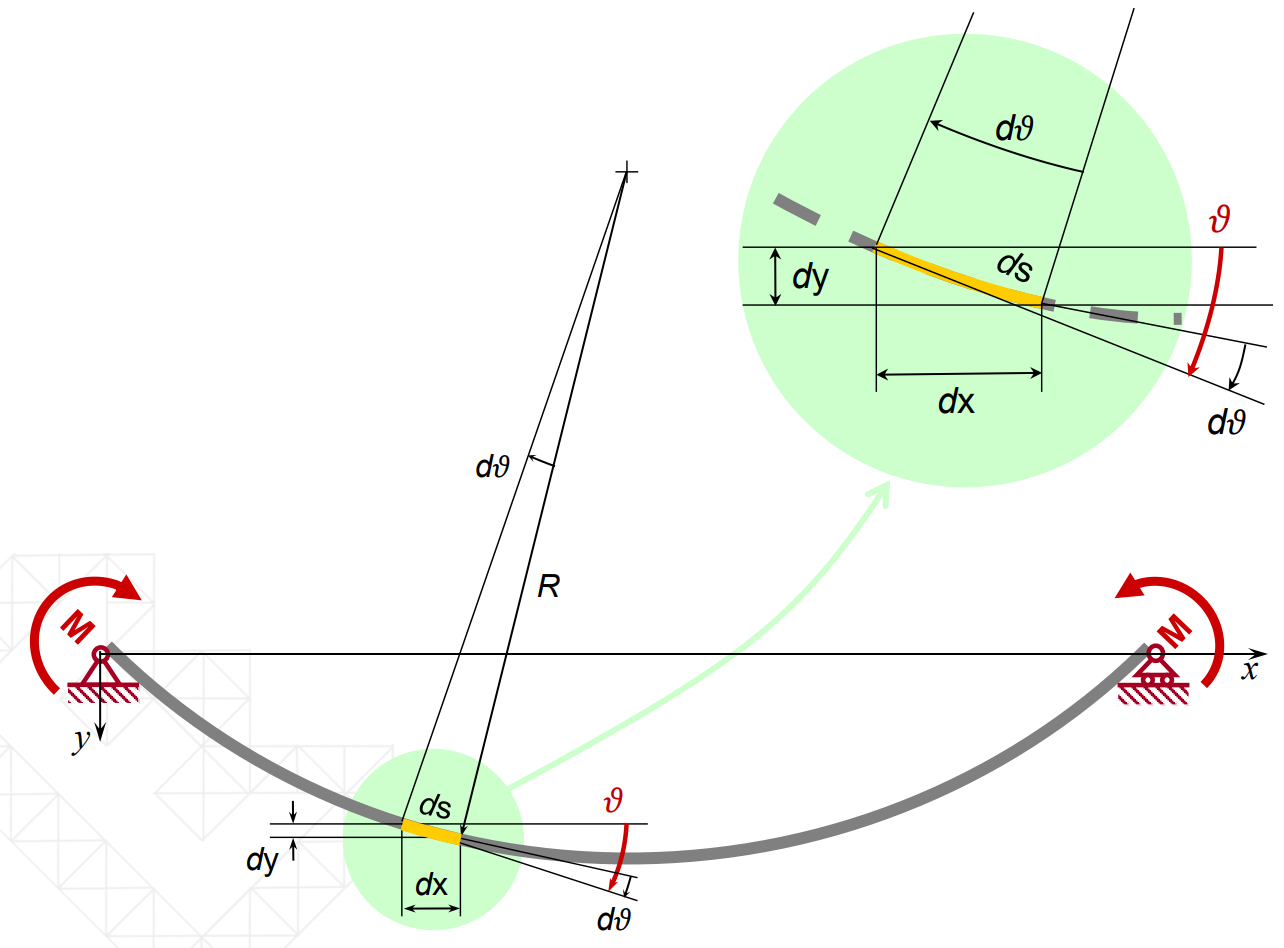
\includegraphics[width = 0.8 \textwidth]{../img/beam2.PNG}
  \caption{The geometry of the beam under bending. The direction of the angle $\theta$ is based on the "right-hand rule".}
\end{figure}
For infinitesimal deformations:
\begin{gather}
  \dif x \approx \dif s = -R\cdot \dif \theta \\
  \frac{1}{R} = -\frac{\dif \theta}{\dif x}
\end{gather}
The negative sign comes from the situation that the $x$ axis direction is towards right while the angle $(\theta)$ direction is to the left. Hence, they are opposite. Since:
\begin{gather}
  M = \frac{EI}{R} \\
  \rightarrow M = -EI\frac{\dif \theta}{\dif x}
\end{gather}
Assuming anlge $\theta$ is small:
\begin{gather}
  \theta \approx \tan(\theta) = \frac{\dif y}{\dif x}
\end{gather}
\begin{itemize} [noitemsep]
  \item The load $w$ in the $y$ direction is the derivative of the shear force $Q$.
  \item The shear force $Q$ is the derivative of the bending moment $M$. 
  \item The bending moment $M$ is proportional to the derivative of the slope $\theta$.
  \item The slope $\theta$ is the derivative of the deflection $y:\theta = \frac{\dif y}{\dif x}$
\end{itemize}
\subsection{Stresses Due to Shear Force}
The shear force also produces stresses into the section (shear stresses). However:
\begin{itemize}[noitemsep]
  \item They are much lower than bending stresses
  \item They are zero at surfaces, where bending stresses are maximum
  \item Their effect on the deformation is negligible compared to bending stresses
\end{itemize}
In general, neglecting the shear stresses due to the shear force is a good approximation for both the calculation of failure and deflections.
\subsection{Summary of Beam Bending Equations}
\textbf{Deflection:}
\begin{gather}
  y
\end{gather}
\textbf{Slope:}
\begin{gather}
  \theta = \frac{\dif y}{\dif x}
\end{gather}
\textbf{Bending Moment:}
\begin{gather}
  M = -EI\frac{\dif \theta}{\dif x} = -EI\frac{\dif^2y}{\dif x^2}
\end{gather}
\textbf{Shear Force:}
\begin{gather}
  Q = \frac{\dif M}{\dif x} = -EI\frac{\dif^3y}{\dif x^3}
\end{gather}
\textbf{Load Distribution:}
\begin{gather}
  w = -\frac{\dif Q}{\dif x} = EI\frac{\dif^4y}{\dif x^4}
\end{gather}
The equations above give a scenario of being given deflection $y$, and eventually finding load distribution $w$. However, the inverse can also occur where load distribution $w$ is given, and the $y$ can be found through integration: \\\\
\textbf{Load Distribution}
\begin{gather}
  w
\end{gather}
\textbf{Shear Force:}
\begin{gather}
  Q = -\int w \cdot \dif x
\end{gather}
\textbf{Bending Moment:}
\begin{gather}
  M = \int Q \cdot \dif x = -\int \int w \cdot \dif x \dif x
\end{gather}
\textbf{Slope:}
\begin{gather}
  \theta = -\frac{1}{EI}\int M \cdot \dif x = \frac{1}{EI}\int \int \int w \cdot \dif x \dif x \dif x
\end{gather}
\textbf{Deflection:}
\begin{gather}
  y = \int \theta \cdot \dif x = \frac{1}{EI}\int \int \int \int w \cdot \dif x \dif x \dif x \dif x
\end{gather}
\subsection{Direct Integration Method}
\subsubsection{STEP 1: Determination of Support Reactions}
Apply to the body the force and moment equilibrium equations to find support reactions (it is possible only if the system is statically determinate).
\subsubsection{STEP 2: Determination of Deflection}
\begin{enumerate}
  \item Write bending moment expression
  \item Use double integration on bending moment expression. This would result in 2 constants of integration.
  \item Use boundary conditions to determinate constant of integration.
\end{enumerate}
\subsubsection{Example: Uniformly Distributed Load on a Cantilever Beam}
\begin{figure}[H]
  \centering
  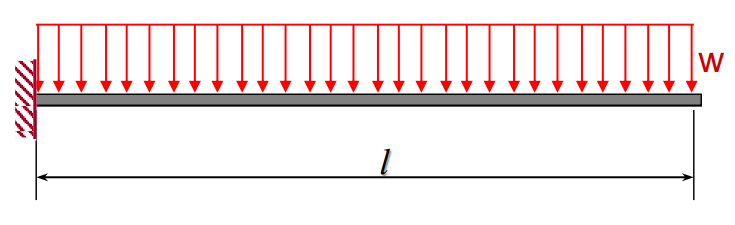
\includegraphics[width = 0.8 \textwidth]{../img/beam3.PNG}
\end{figure}
\textbf{Determination of Support Reactions:}
\begin{figure}[H]
  \centering
  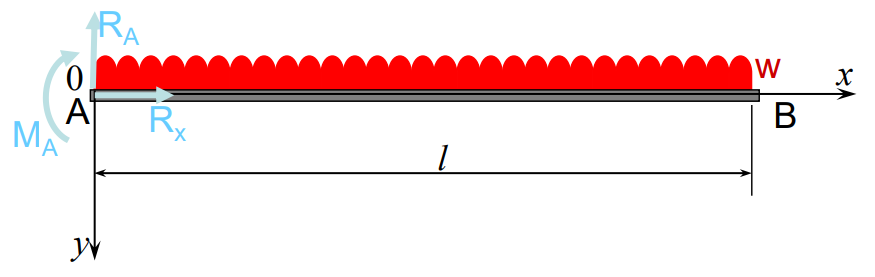
\includegraphics[width = 0.8 \textwidth]{../img/beam4.PNG}
\end{figure}
\begin{center}
  $\vec{R_A} = \left[ \begin{array}{ccc} R_x \\ R_y \\ M_A \end{array}\right]$
\end{center}
\begin{gather}
  \sum F_x: R_x = 0 \\
  \sum F_y: R_y = wl \\
  \sum M: M_A + wl\frac{l}{2} = 0 \\
  M_A = -\frac{wl^2}{2}
\end{gather}
\textbf{Determination of Deflection:}
\begin{figure}[H]
  \centering
  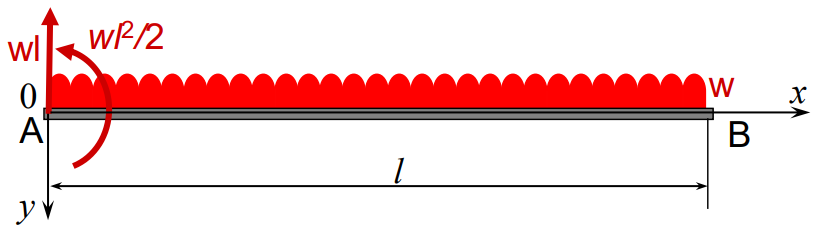
\includegraphics[width = 0.8 \textwidth]{../img/beam5.PNG}
\end{figure}
Direct Integration:
\begin{gather}
  Q = -\int w \cdot \dif x = -wx + Q_0 \\\\
  M = \int Q \cdot \dif x \\
  = \int (-wx + Q_0)\dif x \\
  = -\frac{1}{2}wx^2 + Q_0x + M_0
\end{gather}
Boundary Conditions:
\begin{gather}
  Q(0) = R_y = wl \\
  \rightarrow Q_0 = wl \\
  M(0) = M_A = -\frac{1}{2}wl^2 \\
  \rightarrow M_0 = -\frac{1}{2}wl^2
\end{gather}
Therefore:
\begin{gather}
  Q = -w(x+l) \\
  M = -\frac{1}{2}wx^2 + wlx - \frac{1}{2}wl^2
\end{gather}
Relating Deflection to the Bending Moment:
\begin{gather}
  M = -\frac{1}{2}wx^2 + wlx -\frac{1}{2}wl^2 \\
  \theta = -\frac{1}{EI}\int M \cdot \dif x = -\frac{1}{EI} \left(-\frac{1}{6}wx^3 + \frac{1}{2}wlx^2 - \frac{1}{2}wl^2x \right) + \theta_0 \\
  y = \int \theta \cdot \dif x = -\frac{1}{EI} \left(-\frac{1}{24}wx^4 + \frac{1}{6}wlx^3 - \frac{1}{4}wl^2x^2 \right) + \theta_0x + y_0 \\
\end{gather}
Boundary Conditions:
\begin{gather}
  \theta(0) = 0 \rightarrow \theta_0 = 0 \\
  y(0) = 0 \rightarrow y_0 = 0
\end{gather}
Therefore:
\begin{gather}
  y = \frac{1}{EI} \left(\frac{1}{24}wx^4 - \frac{1}{6}wlx^3 + \frac{1}{4}wl^2x^2 \right) \\
  y_{max} = y(l) = \frac{wl^4}{8EI}
\end{gather}
\end{document}